\chapter{CellTAN: Cellular Time Activation Networks} \label{chap:chap4}

Distributed information systems characterized by time series data present various challenges, primarily due to their complex and dynamic nature. The sheer volume of data that must be processed and analyzed in real time is a significant challenge, leading to concerns over storage, computation, and scalability. Moreover, data quality issues such as missing or incomplete data and data heterogeneity arising from sourcing data from disparate sources with varying consistency and structure further exacerbate these challenges. Another critical challenge of these systems is handling the temporal aspects of time series data, requiring specialized pre-processing, feature extraction, and modeling techniques. The distributed nature of these systems further complexifies matters, with issues encompassing data synchronization and accuracy being a common concern. Furthermore, their implementation in real-world applications requires robust mechanisms for data security and privacy, which adds a layer of complexity to the design and implementation of these systems.

\begin{figure}[h!]
    \centering
    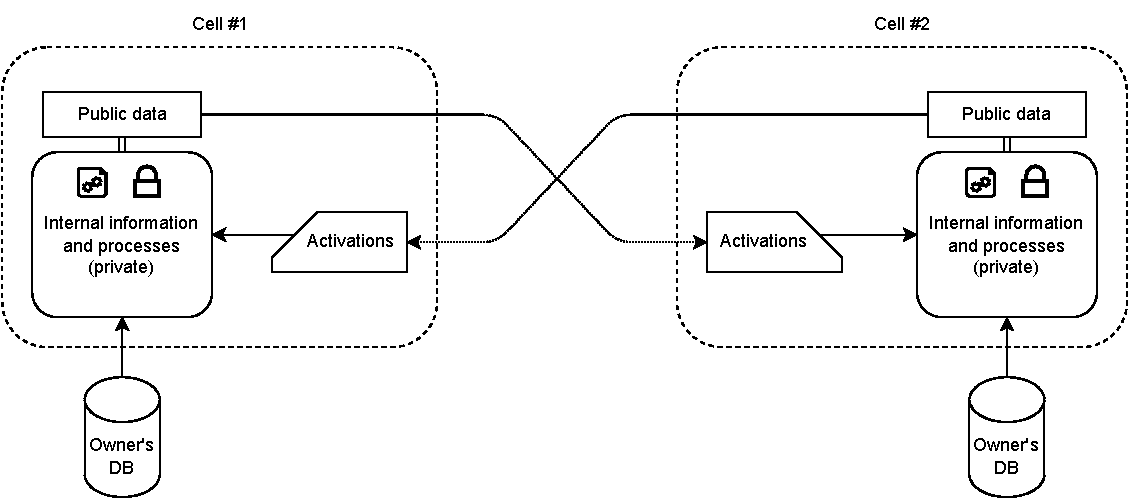
\includegraphics[width=0.9\textwidth]{figures/chapter4/cell/intro.pdf}
    \caption{Simples CellTAN Network of two cells cooperating.}
    \label{fig:celltanintro}
\end{figure}

This chapter proposes a novel tool entitled CellTAN (Cellular Time Activation Network) that undertakes those challenges. CellTAN represents sparse yet interconnected components that function independently, cooperatively, and asynchronously. Inspired by other effective mechanisms like GNNs, CXNs, and Weighted Cross-Connection Networks (WCCNs), CellTAN uses a graph-like structure to represent a network of components with nodes and connections. Following the introductory chapters, its primary purpose is to detect abnormal scenarios on PV systems. However, its generalized formulation introduces other valuable features which come naturally from fulfilling this goal. Such are state estimation, forecasting, and capturing the value in data from different PV asset owners without violating their privacy. For briefness' sake, we will unfold details about its benefits during the rest of this chapter.

Instead of tackling fault detection and classification in a classical centralized manner, which is already extensively showcased throughout the literature, this tool approaches this problem with a paradigm change: a distributed and asynchronous data coherence system. By having a virtual representation closely related to the physical form of sparse systems, we can leverage the relationships between components to assess their correct (or incorrect) operation. While initially designed for photovoltaic (PV) systems, the concepts of cells, connections, neighbors, time series, and uncertainty are universal and applicable to other fields such as biology, physics, and more. Thus, the potential for generic applicability sparks the interest to not bake specifics of PV systems directly into this tool, allowing its usage for other subjects. Figure \ref{fig:celltanintro} represents a minimal scenario for a network: only two cells. It showcases some terms specific to this tool that might be difficult to grasp initially, such as trust, events, and activations. Consequently, detailed explanations throughout this chapter serve to clarify them.

Vast and scattered information across multiple agents is a common scenario faced by the industry of AI for energy systems, which cannot be aggregated due to privacy and confidentiality reasons. Nevertheless, its conjunction could have a lot of added value, given the similarity of certain assets: PV plants (as well as wind farms) from different owners in neighboring geographical regions. This information-sharing potential for AI algorithms motivates the development of a mechanism that communicates information between differently owned assets without any of the compromises above. However, as stated before, data acquisition in PV scenarios is scarcely synchronous and might only occur in equal time resolutions for some of the different components. The CellTAN addresses these issues with an instrument called \textbf{Activations}. It proposes a new way of communication that decouples from the needs of units, sampling rate, and synchronization, avoiding resampling, normalization, or even obfuscation (to protect privacy), by only transmitting time values. This mechanism is a core feature of the tool since it will be the means that will allow connecting different stakeholders' data, and section \ref{sec:thecell} develops this matter thoroughly. Likewise, succeeding sections formulate the working of the cell and its interactions within the network. Since it is the core component, understanding its behavior is crucial for a complete understanding of the tool.

% \section{Glossary} \label{sec:glossary}


% \begin{itemize}
%     \item \textbf{Knowledge base}: Refers to registered historical knowledge (samples) of time series variables.

%     \item \textbf{Inputs}: Uniform fuzzy numbers (not necessarily, but it is the current choice) that represent one sample of the group of time series variables that define the state of a cell.

%     \item \textbf{Outputs}: Similar to inputs, but obtained through some computations.

%     \item \textbf{Time decay}: A process associated with increased uncertainty of variables over time.

%     \item \textbf{Activations}: Timestamps of past occurrences on a knowledge base with a non-zero membership value against a set of recent inputs.

%     \item \textbf{Trust}: A decimal number that represents how coherent two activations are with each other.

%     \item \textbf{Hub}: The central component of the cell network, which facilitates its visualization, management, and expansion. It acts as the proxy agent between the cell's communication.

% \end{itemize}

\section{The Cell} \label{sec:thecell}

% TODO falta mencionar que o dono da célula é que é responsável por estabelecer conexões

\subsection{Principles}

A cell is an independent entity composed of \textbf{data} and \textbf{processes}. The idea is to abstract fundamental system components (e.g., inverters, MPPTs) into this virtual entity. With an added intelligence layer and featuring a few different processes, it assesses its current state based on all available internal and external information, adding value to the existing data acquisition and monitoring systems. As an individual part of the system, it follows a set of rules that define its intrinsic and extrinsic behavior. These rules address data privacy, request boundaries, and real-world operational limitations.

\paragraph*{Independence} During operation, independence on neighbors or other network entities for continuous processing of outputs results in a more robust system and increases cell availability. Thus, given any connection cutoffs, the cell shall be unbothered by its surroundings and continue operating in an isolated state. Isolation is not preferred, but enduring it until outside contact is re-established avoids shutdown and startup procedures.

\paragraph*{Selfish Computations} The cell is selfish in that it will not perform any computations based on the request of others. This aspect creates a fundamental layer of protection against overloading the infrastructure in which it is deployed, which also increases availability.

\paragraph*{Data accessibility} Although selfish in computations, the cell shall provide access to select data valuable to the network. However, not all internal data is shared, and public data shall not compromise the cell's privacy (more on this later).

\subsection{Processes and Data}

The cell's core is a loop of processes that runs periodically. The cell starts in standby mode \textcircled{\raisebox{-0.9pt}{a}}, which is only left when new information arrives or a predetermined amount of time has passed. This mode ensures no unnecessary computational burden of repeating all processes without new data. Nonetheless, by defining a maximum sleep time, we ensure that the cell's public attributes better represent its current state. Figure \ref{fig:cellprocesses} illustrates all its processes and data in a flowchart that goes over its loop from top to bottom. The symbol on the top right of some attributes indicates which persist in the cell's database, and the circular letter tags (e.g. \textcircled{\raisebox{-0.9pt}{.}}) serve to reference specific steps in the following paragraphs,

After receiving new data (inputs \textcircled{\raisebox{-0.9pt}{b}}), the cell enters the computing "activations" phase \textcircled{\raisebox{-0.9pt}{c}}. This procedure relates to temporal similarity extraction, presented in section \ref{subsec:tempsim}. It is associated with searching for similar behavior (of the inputs) in the cell's knowledge base \textcircled{\raisebox{-0.9pt}{z}}, generating "time activations" \textcircled{\raisebox{-0.9pt}{d}}, which are the timestamps of these similar occurrences.

Consequently, the cell starts fetching neighbors' activations \textcircled{\raisebox{-0.9pt}{e}}: an asynchronous process that uses the hub to communicate with other cells. This process only occurs after checking what neighboring cells have activations not older than an acceptable threshold (configured by the cell owner) and if their knowledge bases intersect with the cell's own. However, if a neighborhood of cells receives new inputs simultaneously, it would result in some trying to continue computations while others still do not have activations. Thus, this process checks for neighbors with updated activations up to three times, with a pause in-between, when the current amount does not reach a predefined threshold.

The cell executes a trust computation neighbor-wise \textcircled{\raisebox{-0.9pt}{f}} and variable-wise \textcircled{\raisebox{-0.9pt}{g}} after gathering all neighbor's activations \textcircled{\raisebox{-0.9pt}{h}} and getting new inputs \textcircled{\raisebox{-0.9pt}{a}} (respectively). In practice, this procedure generates a decimal value between zero and one for each input variable and neighbor, which describes how much that variable is coherent with the rest \textcircled{\raisebox{-0.9pt}{i}} and how much a neighbor is coherent with the cell \textcircled{\raisebox{-0.9pt}{j}} (respectively). We nicknamed it "trust" to have a friendlier term used throughout the development and reasoning that unrolls in section \ref{subsec:trust}. This indicator is stored in the owner's database to perform an aggregated analysis related to the "checking historical trust" process \textcircled{\raisebox{-0.9pt}{k}}\textcircled{\raisebox{-0.9pt}{l}}.

The cell reviews past trust data and flags any inconsistencies in trust values during specific periods for variables \textcircled{\raisebox{-0.9pt}{k}}and neighbors \textcircled{\raisebox{-0.9pt}{l}}. If the mean value fall below the owner's threshold, they are flagged and recorded, along with information about the elements and time frames involved \textcircled{\raisebox{-0.9pt}{m}}\textcircled{\raisebox{-0.9pt}{n}}. It raises the severity of the inconsistency accordingly.

Following the activation and trust computations, the cell calculates its output \textcircled{\raisebox{-0.9pt}{o}} \textcircled{\raisebox{-0.9pt}{p}}. It filters its knowledge base \ using intrinsic and neighbor activations and determines the domain of new variables. This process, explained in section \ref{subsec:inout}, also reveals the severity of any unconformity \textcircled{\raisebox{-0.9pt}{o}} that may arise when the activations of variables and neighbors do not intersect. More information can be found in section \ref{sec:states}.

After completing all internal processes, the cell checks if its internal state has changed since the previous loop and updates it \textcircled{\raisebox{-0.9pt}{r}}. This state's information \textcircled{\raisebox{-0.9pt}{s}} concerns the unconformities that it experienced (\ref{sec:states}).

Additionally, the cell may run application-specific plugins \textcircled{\raisebox{-0.9pt}{t}}. These are external additions that the owner might include for uncovering specific situations \textcircled{\raisebox{-0.9pt}{u}} related to the cell's inputs. Further detailed in section \ref{subsec:plugins}, this mechanism binds system logic to the cell and takes advantage of its known physical properties and behavior.

\begin{figure}[h!]
    \centering
    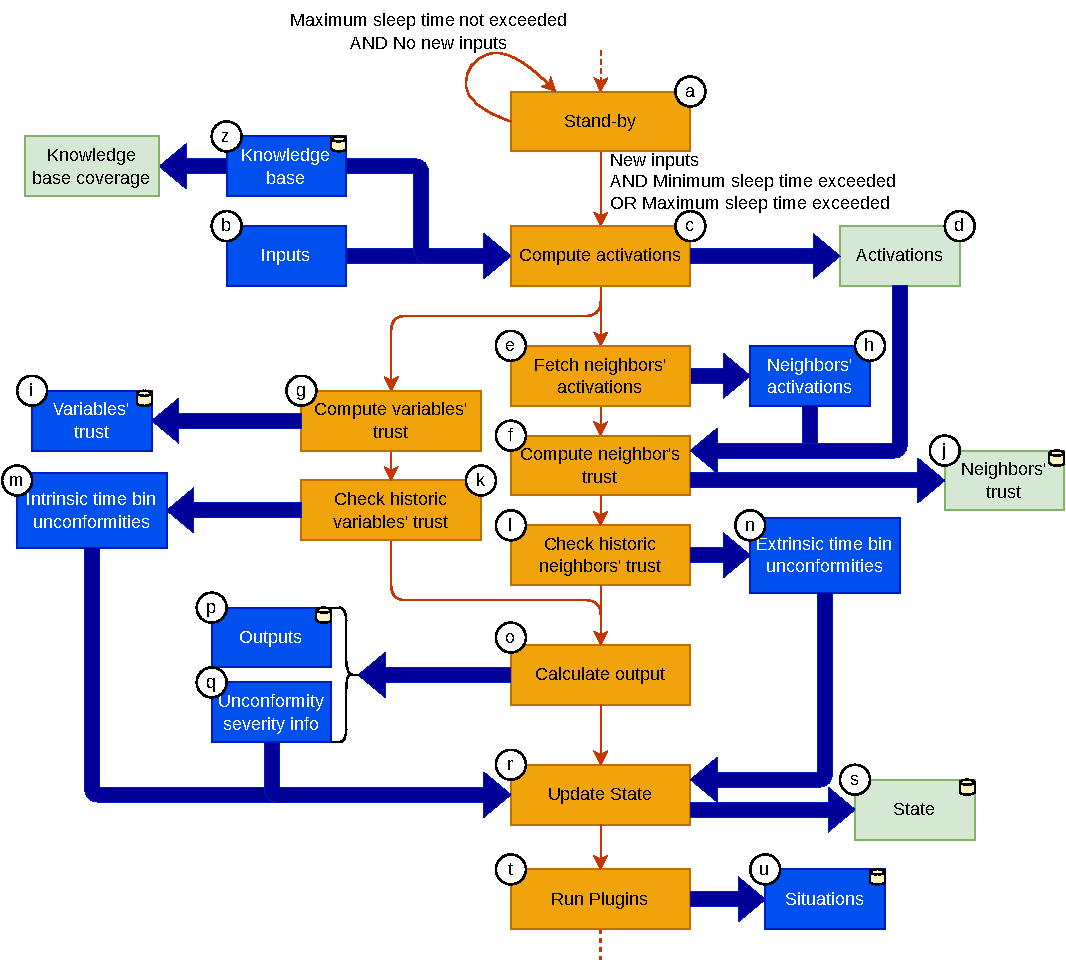
\includegraphics[width=\textwidth]{figures/chapter4/cell/processes.pdf}
    \caption{The cell's core sequence of processes (colored orange) and flow of data (colored blue for private and green for public attributes).}
    \label{fig:cellprocesses}
\end{figure}

Regarding the color coding in figure \ref{fig:cellprocesses}, we can see that most of the cell's attributes are private. The network can access its activations, knowledge base coverage, neighbors' trust, and state. Conversely, the cell extracts neighbors' activations from the network and gives its owner exclusive access to inputs, outputs, knowledge base, and others. The relationship between the owner and private cell data is bidirectional since it is also his responsibility to update the inputs (optimally with an autonomous process). The cell's knowledge base may only represent an interface with a private database (thus a bidirectional connection), not the data itself, since the owner might prefer a centralized storage server instead of storing it within the hardware of the cell.

\subsection{Inputs and Outputs} \label{subsec:inout}

Inputs and outputs are a view of the values that define a cell's variables at a given rolling timestamp. While inputs are directly associated with raw sampled data from the system (injected by the owner), outputs are a byproduct of internal processes. The latter should present more accurate information since it is based on internal and external data (ideally, but not necessarily).

We defined inputs and outputs using classical sets instead of crisp values, which will be crucial for the cell's inner workings. Representing the cell's variables in a fuzzy (or probabilistic) manner can better capture the inherent uncertainty in time series data. However, they are not limited to this representation, with fuzzy numbers or probability distributions as alternatives. Besides, they can be subject to a process called \textbf{time decay}, which ensures that the passage of time negatively affects uncertainty (more on section \ref{subsec:timedecay}). This mechanism increases the robustness of the cell by acknowledging the value of time in assessing its current state.

By generalizing the concept of representing uncertainty, the following structures could characterize inputs and outputs:

\begin{itemize}
    \item Classical set: simple uncertainty band (e.g., uncertainty up, down, relative, etc);
    \item Fuzzy number: generalized fuzzy number representation \cite{Zhang2019} (e.g., triangular fuzzy number (a,b,d;h));
    \item Probability distribution: the distribution's characteristics (e.g., mean ($\mu$) and standard deviation ($\delta$) for Gaussian, the mean rate of occurrence ($\lambda$) for Poisson, etc.);
\end{itemize}

\begin{figure}[h!]
    \centering
    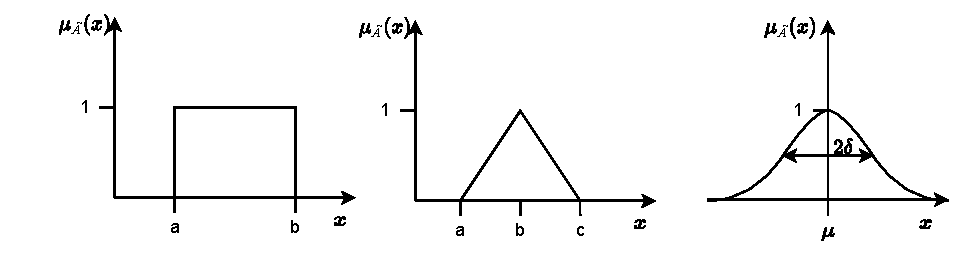
\includegraphics[width=15cm]{figures/chapter4/cell/classic_fuzzy_gaussian.pdf}
    \caption{Classical set, triangular fuzzy number, Gaussian distributions, represented as membership functions.}
    \label{fig:classicfuzzygaussian}
\end{figure}

Classical sets have pros and cons: many operations become more efficient than the alternatives, but we lose density information. Filtering historical data becomes trivial: a value lies within the bounds of the interval (membership value of one) or does not (membership value of zero). This more accessible representation will benefit some cell processes, primarily in temporal similarity extraction (\ref{subsec:tempsim}).

\subsubsection{Time decay} \label{subsec:timedecay}

In real-world dynamic systems that involve data acquisition, the certainty of the data collected tends to fade over time due to its dynamic nature. Typically, the most recent data is the most accurate representation of the system's current state, and as time elapses, the accuracy of previous data points decreases. As a result, it is crucial to consider the time dimension when analyzing dynamic systems and to develop methods that can account for the decay in data certainty over time.

As stated before, and towards considering the time dimension for the current state of a cell, we formulate a \textbf{time decay} method to ensure a more truthful and reliable assessment of the cell's current state. During the standby stage, this process ensures that the inputs and outputs suffer an increase in uncertainty, leading to an uncertain cell in a steady state (without new data input).

Consider the following example of converting a crisp value (5) and uncertainty ($\pm$1) to a classical set:

$$x = 5 \pm 1 \rightarrow [5-1, 5+1] = [4, 6]$$

To simulate the increase in uncertainty over time, we suggest the following equations (\ref{eq:uncertain_down} and \ref{eq:uncertain_up}), applied to each bound:

\begin{equation} \label{eq:uncertain_down}
lower = lower - (lower - minimum) \times \frac{age}{decay}
\end{equation}

\begin{equation} \label{eq:uncertain_up}
upper = upper + (maximum - upper) \times \frac{age}{decay}
\end{equation}

The $age$ variable refers to the time difference between the present time and the instant of data acquisition. For implementation, the time unit considered is the 'second'. The $decay$ is a parametrized constant (same unit as $age$) that defines the time it takes for the set to expand into its limits when starting from the median. It is chosen based on the characteristics of the variable, i.e., knowledge of its uncertainty over time. However, a good starting point is defining close to the data acquisition period so that the set expands entirely until a new value is acquired.

\begin{figure}[h!]
    \centering
    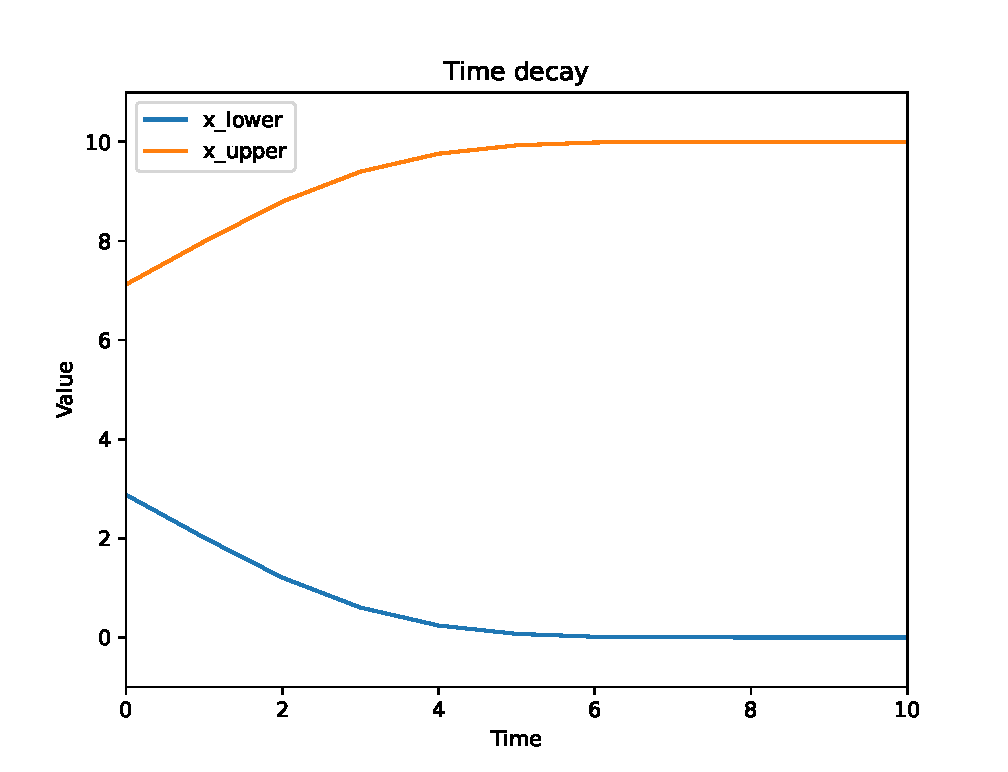
\includegraphics[width=10cm]{figures/chapter4/cell/time_decay.pdf}
    \caption{Visualization of the effect of time decay on $x_{lower}$ and $x_{upper}$.}
    \label{fig:timedecay}
\end{figure}

Figure \ref{fig:timedecay} represents the expansion of the set throughout a period equal to the decay parameter (ten seconds). When the $x$ variable reaches the age of ten seconds, its set representation transmits complete uncertainty: the bounds become similar to the variable limits ($x_{min}$ and $x_{max}$). We can see that the decreasing difference between the bounds and maximum/minimum values causes attenuation in the decay curve, as it displays a non-linear behavior. This behavior seems appropriate according to the reality of systems: as a variable becomes more uncertain with time, there is less potential for its uncertainty to increase.


% \subsection{Temporal similarity extraction} \label{subsec:tempsim}
\subsection{Computing Activations} \label{subsec:tempsim}

Earlier, we brought up the concept of temporal similarity extraction concerning computing activations without fully explaining it. This procedure involves identifying recurring patterns in a statistical base,i.e., finding past instances where we observe the current state to extract useful information about the system's behavior over time. By identifying historical periods with similar conditions, temporal similarity extraction can help assess the current state or predict future trends. This technique of historical search is not exclusive to this application, with demonstrations of use in other fields and for other purposes.

Using sets or probability distributions to filter historical data is one approach to simplify the process of temporal similarity extraction in multivariate time series data while also making it more robust against noisy or incomplete data. This approach assigns membership values to each data point in the time series based on the corresponding set (or distribution) generated from the current cell inputs. We form a group of similar past instances by eliminating samples past a certain threshold. This technique is one of the reasons for deciding to represent the inputs and outputs of the cell in a fuzzy manner.

The proposal for similarity extraction in the cell consists of taking the newly received values (inputs) of the cell's variables (coming from sensors or other data acquisition equipment, calculations, forecasting, etc.), generating a classical set, fuzzy number, or probability distribution from them, and then applying the bounds/membership function or probability density function to the knowledge base (see figure \ref{fig:solo_state_estimation}). If historical samples are associated with membership values, there may be a process for determining outputs by combining data and membership values.

\begin{figure}[h!]
    \centering
    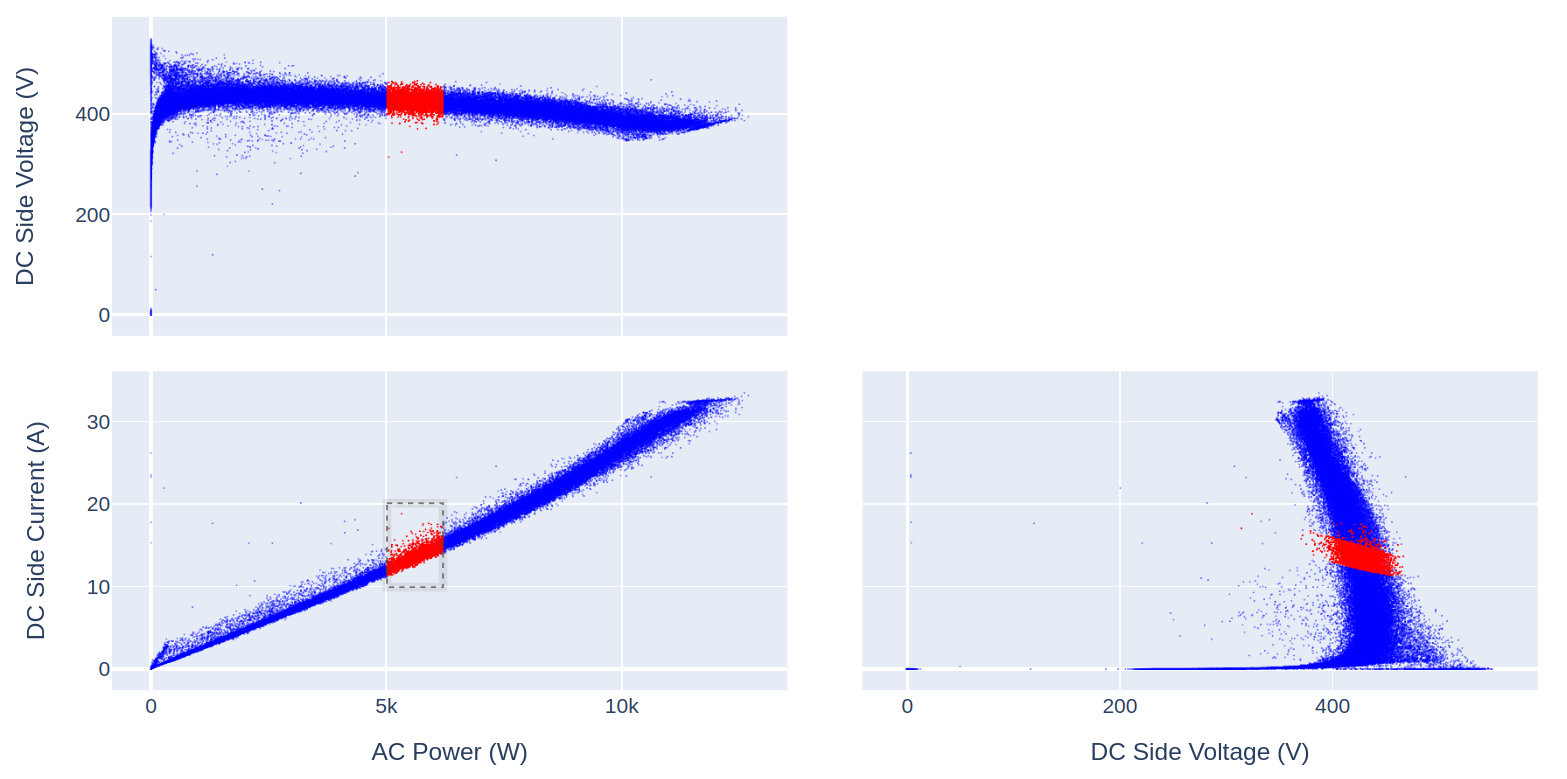
\includegraphics[width=\linewidth]{figures/chapter4/cell/time_extraction.png}
    \caption{Visualization of set-based filtering on example inverter data.}
    \label{fig:time_extraction}
\end{figure}


The initial choice is to use classical sets since filtering history becomes trivial and efficient: restrict the knowledge base to samples where all variables belong to the corresponding interval. Figure \ref{fig:time_extraction} demonstrates a concrete example of this filtering by showing the selected space when filtering by an interval of AC power and AC side current. Generating outputs with this filter can be as simple as constructing a new set based on the bounds of filtered regions (samples with membership equal to one). When filtering historical data with two or more variables, there is a trend of narrowing down the resulting data's space due to the intersection of constraints. Therefore, this process should result in sets that are an equal or better assessment of the present state (than the sets generated by inputs). However, filtering might also result in zero samples (membership value of zero on all knowledge base's rows), which indicates not having "memory" of any similar occurrence. This zero-sample filter is an excellent indicator for potentially anomalous scenarios, primarily if we know that the knowledge base is statistically representative of the variables in the cell (its use is mentioned in \ref{sec:states}).


This process also enables simple forecasting. Considering an offset (arbitrary number of rows/time forward) in the activations, the temporal similarity extraction and computation of outputs results in future values. So, cells may compute outputs related to the present or future. Nonetheless, this temporal shift might be difficult to achieve if data samples arrive at randomly spaced intervals of time, thus would only be straightforward for systems with time-consistent data acquisition.

Up next are practical examples of the temporal similarity extraction methodology. We consider that $t=0$ is associated with the present, and $\mu$ represents membership functions.

\paragraph{Self-similarity}

The cell can perform intrinsic temporal similarity extraction with its knowledge base and input variables. Consider a cell characterized by two variables that are a function of time: $x(t)$ and $y(t)$.
Let us assume that, at a given instant, these are the cell's new inputs:

\begin{equation}
    x(0) = 1.0 \rightarrow \mu_{x(0)}(x) =
    \begin{cases}
        1, & x \in [0.9, 1.1]    \\
        0, & x \notin [0.9, 1.1] \\
    \end{cases}
\end{equation}

\begin{equation}
    y(0) = 2.0 \rightarrow \mu_{y(0)}(y) =
    \begin{cases}
        1, & y \in [1.8, 2.2]    \\
        0, & y \notin [1.8, 2.2] \\
    \end{cases}
\end{equation}

The membership functions $\mu$ are generated considering that $x$ and $y$ are characterized by uniform and symmetrical uncertainty and that the received samples of $x(0)$ and $y(0)$ represent their median (classical set representation).

\begin{figure}[h!]
    \centering
    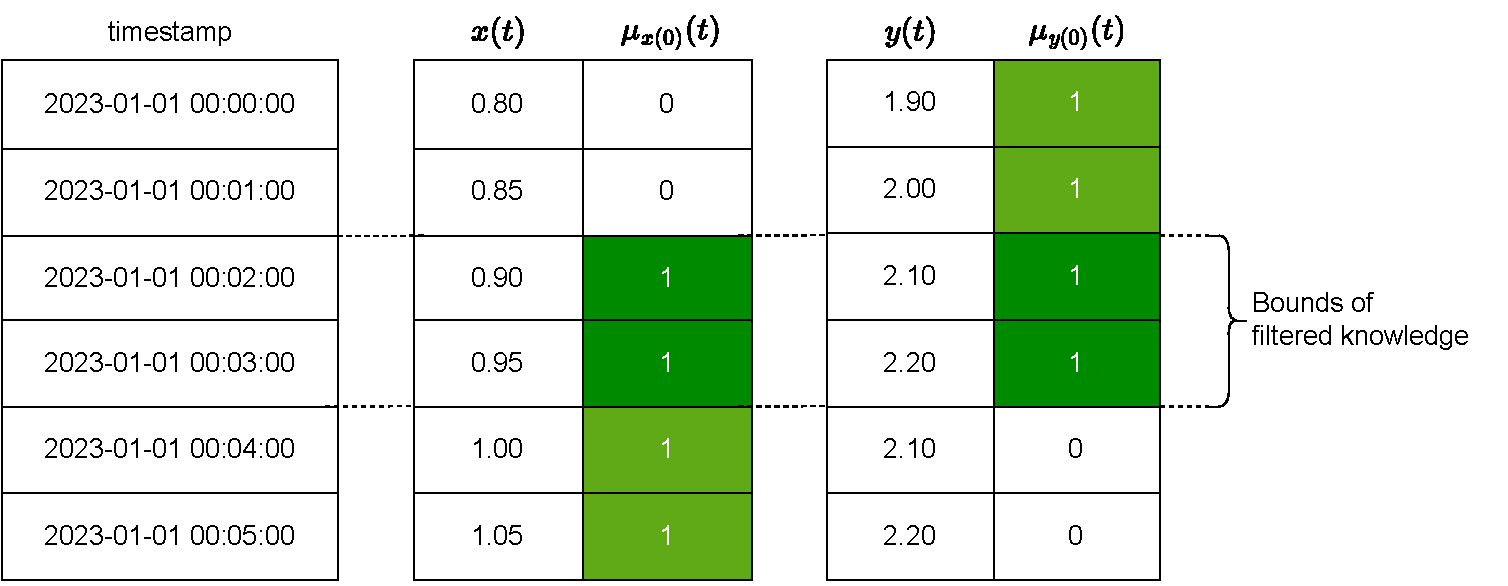
\includegraphics[width=\linewidth]{figures/chapter4/cell/solo_state_estimation.pdf}
    \caption{Visualization of a self-similarity extraction example.}
    \label{fig:solo_state_estimation}
\end{figure}


With the knowledge base represented in figure \ref{fig:solo_state_estimation}, the resulting activations will be 2023-01-01 00:02:00 and 2023-01-01 00:03:00. These are the timestamps of past instances where the cell's variables have values belonging to the set generated from new inputs. Now we can also infer that the actual values of $x$ and $y$ should reside in a set constrained by the filtered historical data ($x(t)$ and $y(t)$). Therefore, the outputs based on self-similarity extraction are:

\begin{equation}
    x'(0) \in [0.90, 0.95]
\end{equation}

\begin{equation}
    y'(0) \in [1.80, 2.20]
\end{equation}

These results confirm that we achieve outputs with less uncertainty only depending on this intrinsic process and private data.

\paragraph{Mutual Similarity}

Extending similarity extraction to multiple cells is a relatively trivial process. Suppose a cell has access to another's activations at the same rolling timestamp and for a historical window that intersects its knowledge base. In that case, it can use that information to refine the intrinsic temporal similarity extraction result. Using sets, this can occur with a simple interval intersection of bounds. Although simple, this process has some tricky requirements, such as not allowing a time difference between the computation of membership values of different cells to avoid joining incoherent information and being able to intersect the activations of cells with different data acquisition periods.

% TODO figura sobre algoritmo de compressão

When analyzing the resulting activations of the previous example, we noticed that using the timestamp of each activated row could be simultaneously more efficient and avoid synchronization issues. Firstly, representing activations by an interval of timestamps instead of the individual rows allows compressing consecutive samples into a single interval.
This new representation may or may not improve efficiency since a knowledge base that filters into alternating activations doubles the memory requirement for this representation. However, an interval representation is suitable if inputs are uncertain and result in a large filter.


% Capacidade de estimação de estado intrínsica + extrínsica


\subsection{Trust}  \label{subsec:trust}


After recognizing the potential for mutual time similarity extraction, we formulate a mechanism for understanding coherence between cells before mindlessly intersecting their activations. This unique characteristic of the CellTAN enables its usage without data privacy issues and not requiring data normalization. However, as seen before, the knowledge base must intersect for a time-based comparison to make sense, and it also yields the best results if outliers are absent (for anomaly detection). Besides cell comparison, activations also allow comparing variables by performing similarity extraction with a subset.

Time possesses inherent normalization properties, as all components equally experience it. This characteristic enables the network to compare systems without concerns about the specific variables involved. Consequently, this is why the proposed tool could be effectively applied beyond PV applications, showcasing its ability to generalize across various domains.

\subsubsection{Trust between Cells}

A 2x2 contingency table represents the intersection of activations of two cells. In this table, the rows define the activation status of one cell (labeled as "Activated" and "Not Activated"), and the columns represent the activation status of the other cell (same labels).

\begin{table}[h!]
    \centering
    \caption{Contigency table representing the activation intersection of two cells.}
    \label{tab:cellactivationsintersection}
    \resizebox{8cm}{!}{%
    \begin{tabular}{ll|cc|}
    \cline{3-4}
    \multicolumn{2}{l|}{\multirow{2}{*}{}} & \multicolumn{2}{c|}{Cell 2} \\ \cline{3-4} 
    \multicolumn{2}{l|}{}                                     & \multicolumn{1}{l|}{Activated} & \multicolumn{1}{l|}{Not Activated} \\ \hline
    \multicolumn{1}{|c|}{\multirow{2}{*}{Cell 1}} & Activated & \multicolumn{1}{c|}{a}         & b                                  \\ \cline{2-4} 
    \multicolumn{1}{|c|}{} & Not Activated & \multicolumn{1}{c|}{c}  & d \\ \hline
    \end{tabular}%
    }
\end{table}

Each element of the matrix represented in Table \ref{tab:cellactivationsintersection} ($a$,$b$,$c$, and $d$) corresponds to a specific combination of activations, such as "Activated-Activated," "Activated-Not Activated," "Not Activated-Activated," and "Not Activated-Not Activated". They represent the frequency or count of observations falling into that specific combination. The main diagonal relates to the cells' agreeableness, while the secondary diagonal is the opposite. For this work, we decided to use the 'second' as the terms' unit, meaning that, for example, $a$ is the total amount of seconds both cells are active.

The matrix representation of the activation intersection metrics resembles the statistical results of sampling a population with two binary categories. Therefore, a statistical test could be appropriate to calculate the association between these categories. The following section develops this topic.

\subsubsection{Statistical tests for measuring association}

In statistics, numerous tests are available to measure the association between variables in contingency tables. One of the most known tests is Pearson's chi-square test (\ref{ap1:pearsonschi}), which assesses whether there is a significant association between the two variables. It compares the observed frequencies in the contingency table with the expected frequencies under an assumption of independence. If this test yields a statistically significant result, it suggests a non-random association between the activations of the two cells.

Another widely employed test is Fisher's exact test (\ref{ap1:fischer}), as an alternative to the chi-squared, which is particularly useful for small sample sizes. It calculates the probability of obtaining the observed distribution of activations in the contingency table, also assuming independence between the variables. If this probability is sufficiently low, it implies that the association between the activations is unlikely to occur by chance. The odds ratio and relative risk can also quantify the strength and direction of the association between two variables. The odds ratio would compare the odds of activation in one cell close to the other, while the relative risk compares the risk of activation in one cell to the risk in the other.

Considering that the desired outcome of activation comparison between cells is a normalized index that translates into how much they conform to each other (hence the term "trust"), there is a preference for inherently normalized tests, such as the $\phi$ coefficient (\ref{ap1:phi}), contingency coefficient (\ref{ap1:contingencyc}), and Theil's U (\ref{ap1:theilsu}). The goal is that this index represents how much the historical incidence of two cells' states match.

The $\phi$ coefficient, also known as Matthews correlation coefficient, is a measure of association designed explicitly for 2x2 contingency tables, quite popular in machine learning for measuring the quality of binary classification. It ranges from -1 to 1, where 0 indicates no association, -1 represents a perfect negative association, and 1 represents a perfect positive association. The contingency coefficient extends this coefficient's usability, allowing its application in larger contingency tables, and ranges from 0 to 0.707 (no association to strong association).
Finally, another relevant test is Theil's U . It accounts for the variables' mutual information and entropy based on information theory principles, providing a measure for the proportion of total entropy in one variable that the other can explain. It also ranges from 0 to 1.

\subsubsection{Proposed trust measurement method for cells}

All the mentioned tests may offer different perspectives on the association between the activations of two cells. However, none are considered adequate for our application, so we propose a new method, defined by \ref{eq:cdmchi}.

\begin{equation} \label{eq:cdmchi}
    \chi_a^{2'} = \frac{(p_a - E(p_a))^2}{E(p_a)}
\end{equation}

Where:

\[
    p_a = \frac{a}{a+b+c+d}
\]

\[
    E(p_a) = \frac{(a + c) \times (a + b)}{(a+b+c+d)^2}
\]

\begin{align*}
    p_a &: \text{Probability of both cells being active} \\
    E(p_a) &: \text{Expected value for the probability of both cells being active}
\end{align*}

Based on Pearson's chi-squared test, this new approach focuses on the "a" component: the pure agreeableness between two cells. Its value ranges from 0 to 1 (no "trust" to complete "trust"). Some of the most relevant tests previously presented, namely the $\phi$ coefficient, contingency coefficient, and Theil's U, are compared to this new method for comparison and validation in the following experiments.

\subsubsection{Experiments and validation}

\paragraph{Experiment nº1}

The first trial simulates the variation of the $d$ component and its effect on some association coefficients. It's expected that, as not activated time increases, the chance of the two cells intersecting activations lowers, and so their trust should increase. The starting point and used spaces of $d$ are:

$$
\begin{bmatrix}
    30 & 10 \\ 10 & d
\end{bmatrix}
$$
$$
d \in [0, 100], d \in [0, 3000]
$$

\begin{figure}[h!]
\centering
    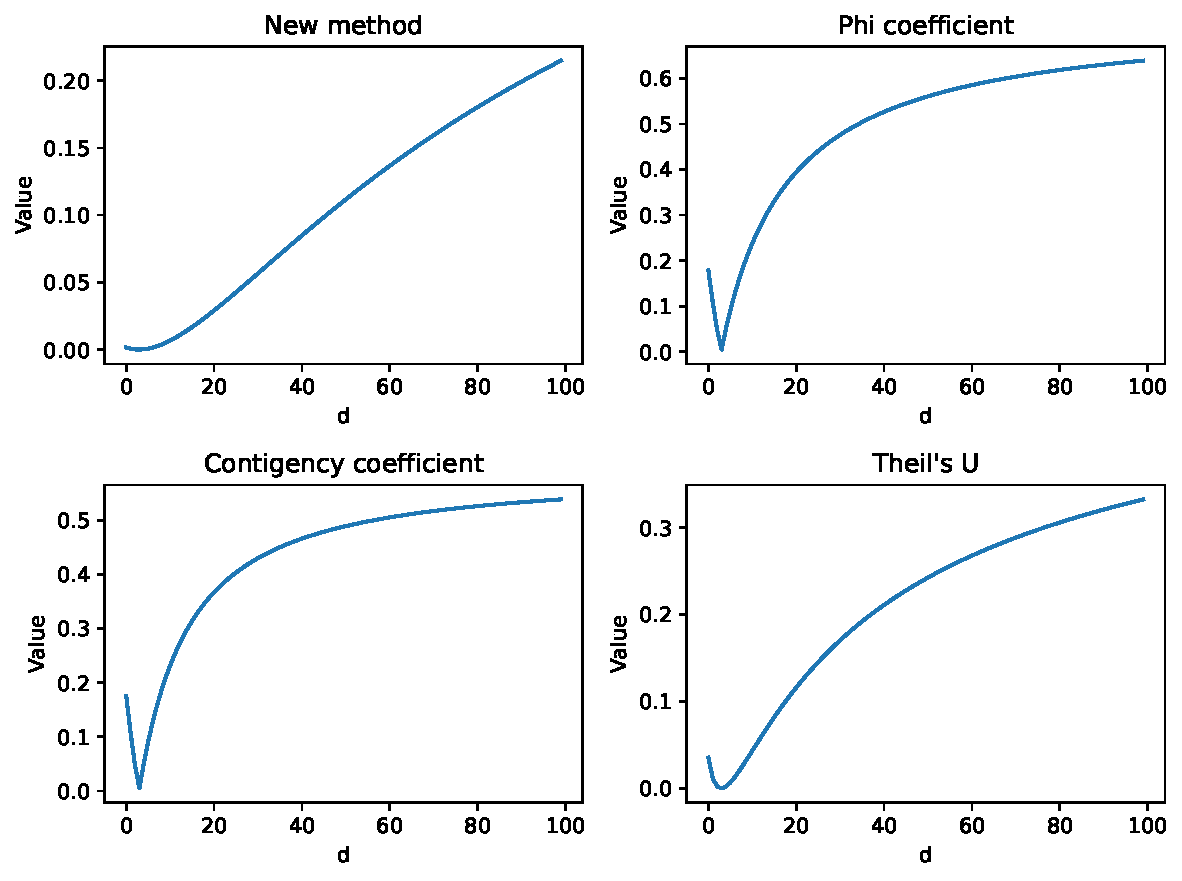
\includegraphics[width=0.8\textwidth]{figures/chapter4/cell/trust_tests/1_a.pdf}
    \caption{Trust measurement evolution for different methods with $a=30, b=10, c=10, d \in [0, 100]$.}
    \label{fig:trust_test_1_a}
\end{figure}
\FloatBarrier


In figure \ref{fig:trust_test_1_a}, we can observe that all measurements increase with $d$, with a slight reduction at the start, although attenuated on the new method. Theil's U's minimum is 0.5, while the expectation for having a lower $d$ (few deactivated intersecting periods) is a value closer to zero (as the other methods demonstrate). This scenario means either both cells have no history similar to current inputs or their inputs' values have significant uncertainty (remember the time extraction process from \ref{subsec:tempsim}). Therefore, their "trust" should be minimal.
Not having a reduction in the first values of $d$, showcased by the new method, is the intended behavior. Having equal activated and deactivated intersections ($a$ and $d$) should not be significantly penalized versus having $a>>d$, justified by the above reasoning.

\begin{figure}[h!]
\centering
    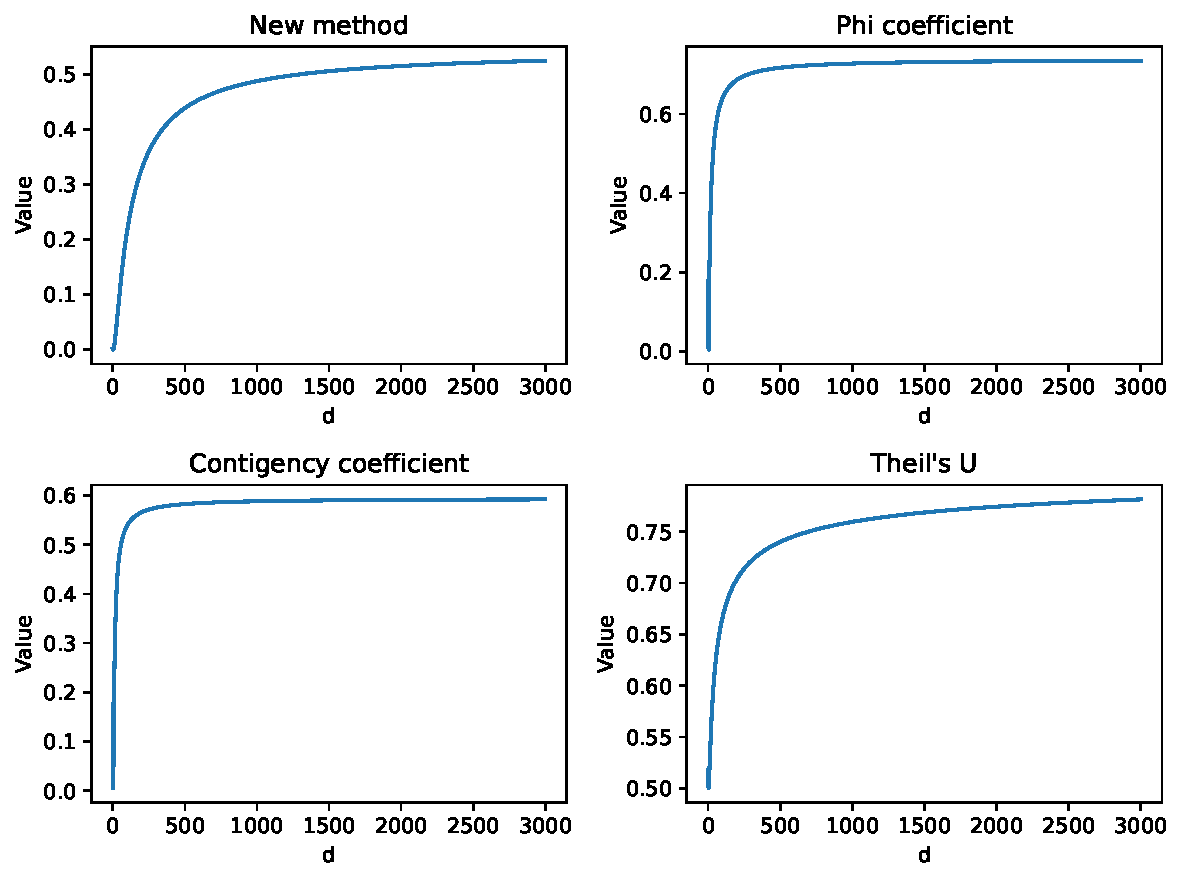
\includegraphics[width=0.8\textwidth]{figures/chapter4/cell/trust_tests/1_b.pdf}
    \caption{Trust measurement evolution for different methods with $a=30, b=10, c=10, d \in [0, 3000]$.}
    \label{fig:trust_test_1_b}
\end{figure}
\FloatBarrier

Figure \ref{fig:trust_test_1_b} extends the previous analysis, showcasing that all methods have asymptotical behavior, settling in a value greater than the start. All except Theil's U have asymptotes deemed acceptable for this test: since disagreement terms $b$ and $c$ are non-null and relatively close to $a$, we expect that the trust index does not reach a value near the max, remaining closer to a measure of "half trust".

\paragraph{Experiment nº2} Now, we observe the impact of the disagreeing terms $b$ and $c$ in the same coefficients by varying one while maintaining all others fixed. The expectation is that an increase in disagreement should lead to zero trust.

$$
\begin{bmatrix}
    30 & b \\ 10 & 10
\end{bmatrix}
$$
$$
b \in [0, 1000]
$$
\begin{figure}[h!]
\centering
    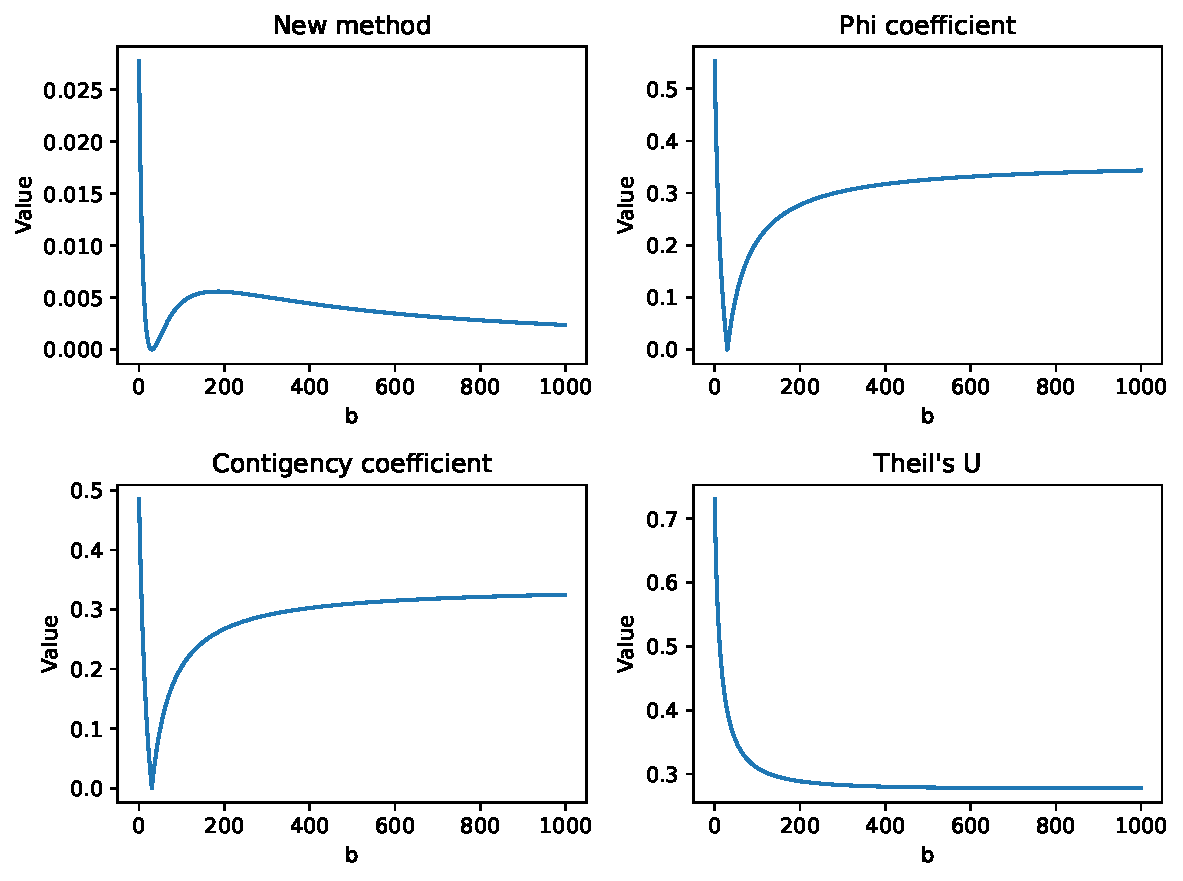
\includegraphics[width=0.8\textwidth]{figures/chapter4/cell/trust_tests/2_a.pdf}
    \caption{Trust measurement evolution for different methods with $a=30, c=10, d=500, b \in [0, 1000]$.}
    \label{fig:trust_test_2_a}
\end{figure}
\FloatBarrier

In figure \ref{fig:trust_test_2_a}, it is clear that, for all methods, an increase in $b$ leads to lower coefficients. All except the new algorithm tend towards similar asymptotes, near a value of 0.3. The new method meets the expected behavior.

$$
\begin{bmatrix}
    30 & 10 \\ c & 10
\end{bmatrix}
$$
$$
c \in [0, 1000]
$$
\begin{figure}[h!]
\centering
    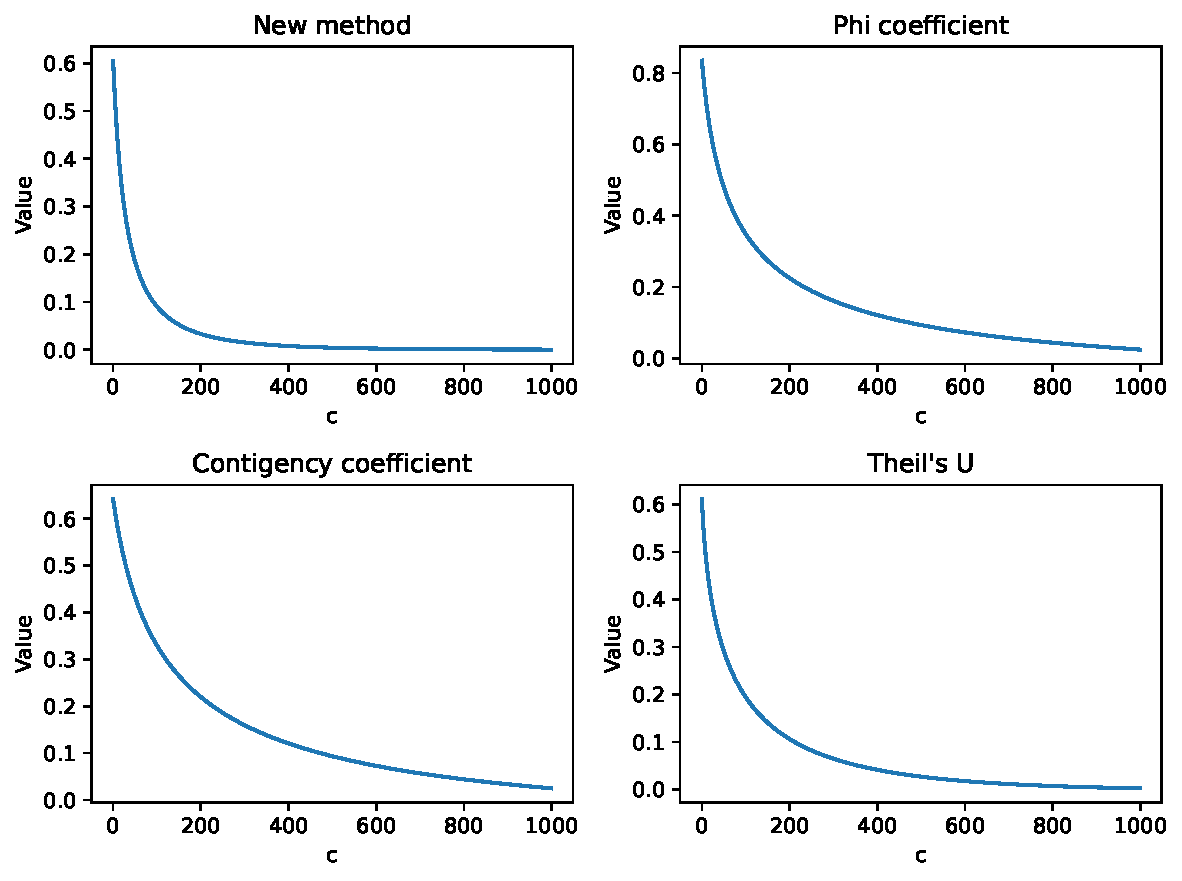
\includegraphics[width=0.8\textwidth]{figures/chapter4/cell/trust_tests/2_b.pdf}
    \caption{Trust measurement evolution for different methods with $a=30, b=10, d=500, c \in [0, 1000]$.}
    \label{fig:trust_test_2_b}
\end{figure}
\FloatBarrier

With figure \ref{fig:trust_test_2_b}, we can observe the asymmetry of Theil's U coefficient, opposing to what figure \ref{fig:trust_test_2_a} showed. It does not represent the trust between cell nº1 and cell nº2, but the trust of cell nº1 \textbf{in} cell nº2. The rest of the methods have symmetrical coefficients, thus presenting the same results.

\paragraph{Experiment nº3} This last experiment showcases the effect of changing term $a$. When the cells share an increasing amount of activated time, assuming their trust should increase is trivial. However, reasoning that having a disproportionally ample activated time means there is more uncertainty on their current state, then trust should lower. The expectation is that, as $a$ increases, there is also an increase in trust until a specific peak. It should decrease after reaching a global maximum and have an asymptote at zero.

$$
\begin{bmatrix}
    a & 10 \\ 10 & 500
\end{bmatrix}
$$
$$
a \in [0, 1000]
$$

\begin{figure}[h!]
\centering
    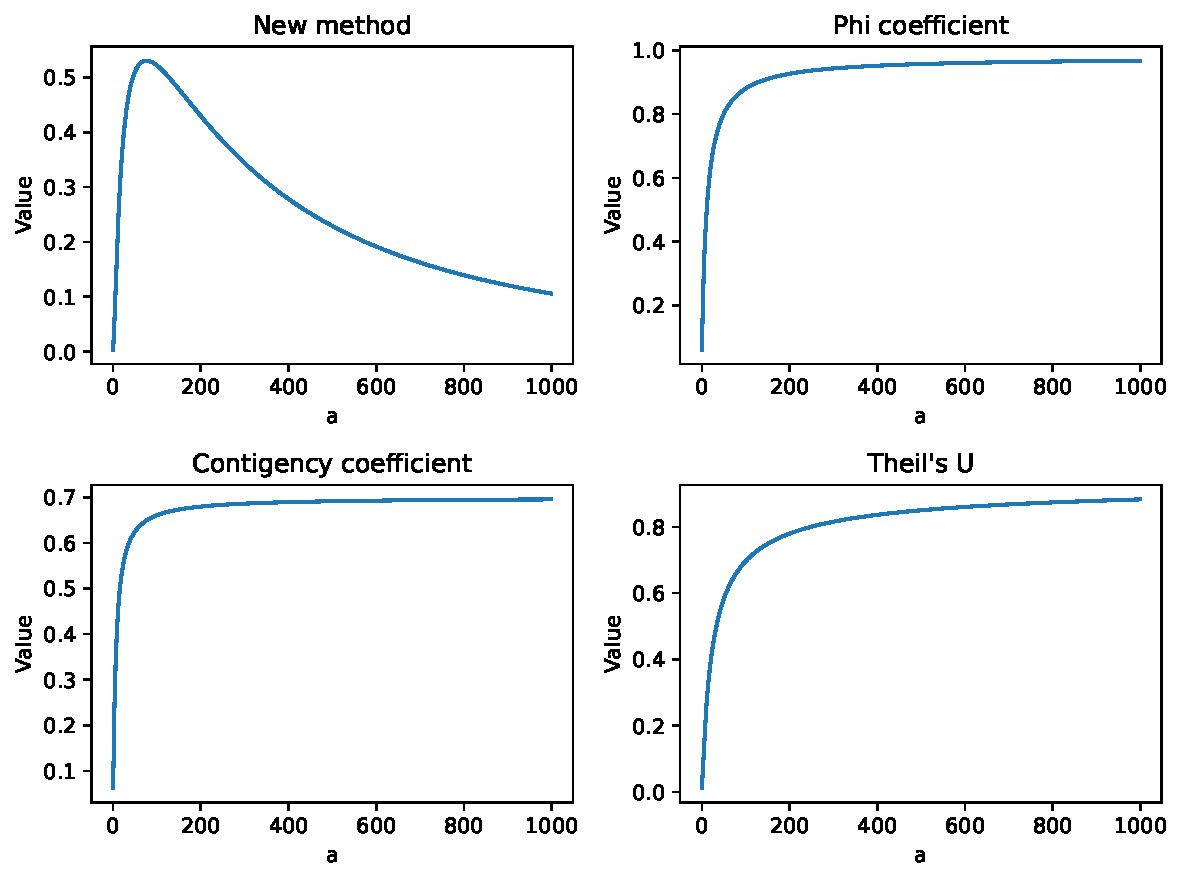
\includegraphics[width=0.8\textwidth]{figures/chapter4/cell/trust_tests/3.pdf}
    \caption{Trust measurement evolution for different methods with $b=30, c=10, d=500, a \in [0, 1000]$.}
    \label{fig:trust_test_3}
\end{figure}
\FloatBarrier

Figure \ref{fig:trust_test_3} shows that only the new method presents the previously described "goal" behavior. Otherwise, all other coefficients approach their max when $a$ tends towards infinity.

With the three experiments presented, we confirm that the proposed approach for computing the trust index between cells is better suited, considering the requirements and assumptions.

\subsubsection{Trust between variables}

Variables defined in the inputs/outputs of the cell can also be subject to activation comparison. Accordingly, we suggest simplifying this process compared to the inter-cell trust \ref{eq:trustvars}. Given that a cell may possess many variables, we restrict this computation to one per each, comparing the activations of a single variable with the intersection of all others.

\begin{equation} \label{eq:trustvars}
    Trust = 1 - \frac{TA_{others, exclusive}}{TA_{self,others} + TA_{self, exclusive} + TA_{others, exclusive}}
\end{equation}

We utilize equation \ref{eq:trustvars} to calculate the trust indicator for variables. The resulting value will be normalized and transparent, reflecting how much a variable was inactive while others were active.

\subsection{Cell Linking}

Mutual similarity extraction and trust calculation cannot occur in isolation. Therefore, connections are the essence of forming the CellTAN. These links can also have indicators for describing the cells' relationships, like the trust index, which is crucial for anomaly detection.

Each cell has a unique identifier, generated upon creation and independent of the name attributed by the owner. This ID serves to register cells and better manage the network. Since interconnections require an agent to keep track of these IDs and correctly redirect traffic, we introduce the \textbf{Hub} component. This central element provides global network visibility and makes connections easier to form and maintain. For a cell, a connection is no more than the identifier of the neighbor, which the hub can directly associate with a communication link.

On cell deployment, the system expects the owner and the CellTAN manager to manually link cells together by assigning each connection. However, the plan is to develop a mechanism that proposes new connections based on the neighbor's neighbors through the hub. This mechanism could function based on the strength of the relationship between cells and neighbors in common, recommending a direct link if both "trust" them similarly. As the last phrase hints, an indicator called "trust" is the criterion for evaluating these links. The following subsection defines the conception of this metric.

\subsection{Unconformities and State} \label{sec:states}

We introduce a state system to expose the resulting unconformities found during cells' processes. These unconformities can categorized into intrinsic and extrinsic, based on the historical check of trust in the variables and neighbors, respectively, and during output computation.

Cells rely on aggregated trust values to assess the integrity and coherence of information. During specific time windows, these systems employ a verification process to identify unconformities in the aggregated trust values. Unconformities are flagged when the aggregated trust values fall below a certain threshold, which the owner predetermines. To establish a framework for this assessment, the owner specifies time bins upon cell creation, which define intervals evaluated from the current rolling timestamp to the past. Consequently, when inconsistencies are detected, detailed information is recorded to identify the elements that exhibit incoherence and the corresponding time bin in which the discrepancies occur. This approach allows for the characterization and analysis of "Intrinsic/Extrinsic time bin unconformities," thereby enabling the system to escalate the severity of unconformities from none to partial or total if some or all elements within a time bin exhibit incoherence.

\begin{figure}[h!]
\centering
    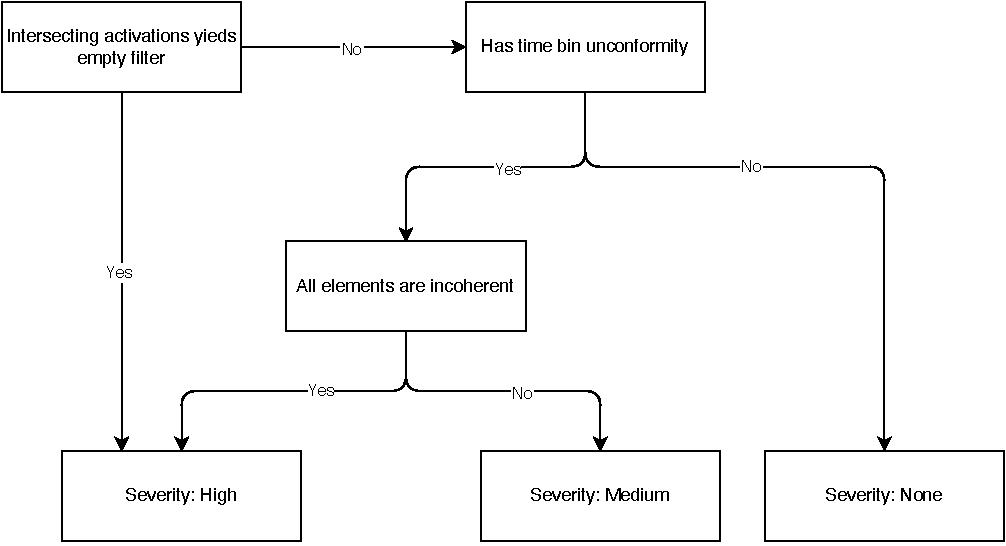
\includegraphics[width=0.9\textwidth]{figures/chapter4/cell/states.pdf}
    \caption{Algorithm for deciding unconformity severity (intrinsic and extrinsic).}
    \label{fig:severity}
\end{figure}

In addition to the assessment methodology mentioned above, intrinsic filtering and the intersection of neighbor's activations play a crucial role in determining the overall unconformity state of the cell. Specifically, suppose intrinsic filtering yields a null domain. In that case, it indicates that the cell has encountered total intrinsic unconformity, suggesting a fundamental breakdown or lack of coherence with its knowledge base. Similarly, suppose the intersection of the neighbor's activations yields a null domain. In that case, it signifies total extrinsic unconformity, implying that the cell lacks trust in its external environment. These higher states of unconformity, whether intrinsic or extrinsic, serve as valuable indicators called the "Unconformity severity info." Considering this additional information, the system can escalate the severity level set by the time bin unconformities, providing a more comprehensive understanding of the cell's overall integrity and the extent of the identified unconformities.

Figure \ref{fig:severity} sums up the algorithm of choosing unconformity severity. The severity level is associated with each type of unconformity since incoherence between neighbors and variables is not necessarily related. The first transition happens during output computation and the time bin unconformities is found during a historical trust assessment (processs seen in figure \ref{fig:cellprocesses}).

Though informative, the meaning of the unconformities and their severities is relatively broad, causing the cell to overlook specific situations related to its physical behavior. The following section addresses this, suggesting an application-oriented approach to extend observability.

\subsection{Application Plugins} \label{subsec:plugins}

% ? Isto devia criar um capítulo inteiro só por sí não?

The broad capabilities of the CellTAN make it less insightful when extracting specific information from the cells. Although its generalized design extends usability to different types of systems, it still requires additional processes to assess particular situations beyond what the state provides. During the literature review process, the specificity of algorithms is noticeable, and most techniques do not attempt to diverge from the PV application when it comes to fault detection and classification. This standard approach yields excellent results and could boost CellTAN's capabilities.

To solve the presented issue and dwell on the PV application theme of this work, we introduce the concept of \textbf{plugins}. Plugins extend the cell's core functionality, introduced to leverage specific system logic to identify patterns in its variables, just like classical algorithms. When binding them to a cell, they have a setup that checks if the required variables are present in its inputs. Then, after the intrinsic processes, they can run an algorithm that assesses what current situation the cell might be experiencing. This way, the CellTAN can still work with entities of different natures while these plugins work alongside, accessing private data and reporting sensible insights to the owner. Nonetheless, they are confined to the cell's scope since permitting access to other cells' variables violates the privacy principle.

To illustrate this feature, let us imagine setting up a CellTAN representative of a solar farm with PV inverter cells. Although the tool does not "know" anything about inverters nor "cares" that the cells are of this type, the agent responsible for adding them to the network certainly does. Therefore, binding a PV-specific algorithm to assess particular inverter situations, such as malfunction, over(/under) voltage(/current), and performance degradation, is wise. This additional process makes the tool warn the owner of specific inverter faults besides possible mismatches in neighboring inverters and variables through the generalized cell procedures. The formulation of a PV plugin, used in a real case study of the CellTAN, happens in chapter \ref{chap:chap5}.

\section{The Hub}

The CellTAN tool is supposed to be easily accessible for different assets and owners in any given location. However, for privacy and security reasons, monitoring equipment and other smart devices (IoT, servers, etc.) in PV plants and the owner's database are usually protected from unwanted outside connections. Because of this, the CellTAN network owner can act as a proxy and be responsible for arranging the necessary connections between the equipment of different asset owners and the network. Routing all traffic through this system may solve previous issues, but introducing a bottleneck will influence availability. This downside is inevitable for aggregating distributed systems and sharing information between otherwise reserved agents. Besides being a proxy, other responsibilities associated with the hub may also be:

\begin{itemize}
    \item Provide network visibility: cells and connections;
    \item Cell connection proposal.
\end{itemize}

% Adding this component permits visualizing all the cells registered in the system and their public data. With this global vision, it may have algorithms 
% % TODO complete

\section{Implementation}

\subsection{Code and Infraestructure}

Materializing both the cell and the hub happened by coding Python modules. It was developed using a mix of the OOP (Object Oriented Programming) and FP (functional programming) paradigms and features a structure familiar with the descriptions in previous sections. Using Python for the implementation of the CellTAN comes with the following advantages:

\begin{itemize}
    \item Easy to read and write code, requiring less syntax for complex operations compared to low-level languages;
    \item Extensive availability of libraries and tools;
    \item Deployment ease: does not have to compile, only needing an interpreter and dependencies to run;
    \item Big community support, with many resources publicly available online (e.g., documentation, tutorials, etc.). 
\end{itemize}

% imagem com as tecnologias em anexos talvez

Docker containers \cite{docker} are the infrastructure choice for deploying these modules (Cells and Hub). They allow running software as containerized applications, with all the necessary dependencies installed in an isolated environment. It acts as a separate system built for running the application instead of relying on the host's OS (Operating System) and running bare-metal. This execution strategy adds an isolation layer between the program and the host machine, increasing safety and making the "production" environment more predictable and stable. An overview of the technology stack utilized (and proposed) for the software products created in this work is pictured in appendix \ref{ap1:techstack}.

% dockerfile em anexos?


\subsection{Communication Protocol}

In the context of ensuring proper data sharing between cells, the choice of communication protocol is a crucial aspect of establishing connections. For this work, we implemented a local communication mode for cells running on the same machine or within the same process and a remote communication model intended for cells distributed across different servers. The local communication mode is straightforward, assuming direct links between cells within the program. However, multiple protocol options regarding remote communication exist, including HTTP, HTTPS, WebSocket, and MQTT (excluding protocols for wireless proximity communication, as the CellTAN system assumes cells may be in different geographical locations). Initially, we implemented HTTP/HTTPS for remote communications due to its accessibility and ease of implementation. However, given its synchronous operation (based on request and response), we soon realized there might be more appropriate and robust choices for a distributed asynchronous system. Consequently, as future work, we should refactor the remote interface to utilize MQTT.

HTTP (Hypertext Transfer Protocol) and MQTT (Message Queuing Telemetry Transport) are communication protocols in different contexts. HTTP, a request-response protocol widely used in web applications, operates over TCP and follows a client-server model. It proves suitable when clients need to retrieve or send specific data to and from a server. HTTP is simple, widely supported, and compatible with browsers and standard web technologies. However, its stateless nature and lack of optimization for real-time communication can result in high overhead caused by frequent request-response cycles.

% TODO referencias

In contrast, MQTT is a lightweight publish-subscribe messaging protocol designed for efficient communication in distributed systems, especially within the Internet of Things (IoT). MQTT utilizes a broker-based architecture, where clients publish messages to topics and subscribe to receive messages from specific topics of interest. MQTT is highly scalable, bandwidth-efficient, and supports asynchronous messaging. It minimizes network and power consumption while providing reliable message delivery. However, implementing MQTT may require additional infrastructure, such as MQTT brokers.
The publish-subscribe model of MQTT facilitates decoupled communication between system components, allowing for scalable and flexible systems. It is suitable for scenarios where devices or services exchange information in a distributed environment asynchronously. MQTT often outshines HTTP as the preferable choice for a distributed asynchronous system emphasizing real-time data exchange and efficient communication. Nevertheless, HTTP remains the more appropriate choice if the system primarily revolves around traditional web applications and request-response interactions. Ultimately, the scope of CellTAN requires the leverage of both protocols in different aspects of the tool: HTTP is more suitable for human-system interaction, and MQTT for system-system exchanges.


\subsection{Cell configuration and deployment}

Configuring cells can be done through configuration files (one per cell). They should contain the cell variables' definitions, database credentials, hub credentials, and all other parameters. Because of its simplicity, we chose the YAML serialization specification \cite{yaml} to parse these configurations. A walkthrough of the cell configuration and expected file structure is present in appendix \ref{ap1:config}


% meter anexo para explicação das configs com screenshot de configuração exemplo
